This tool has been used to verify five BPMN-CWP pairs. The effectiveness of this tool will be measured by both the verification time. Two procedural generated, scalable examples will be used to measure both sequential (many linear decisions) and parallel (many synchronous actors) scalability of this model checking approach.

The first example has been explained thoroughly in \secref{sec:simpleExample}. The rest of the examples will be destribed in this section, along with tables and graphs of results.

\begin{comment}
\figref{fig:face2face_bpmn} shows the BPMN of the first example, a face-to-face purchase. The Buyer and seller are condensed into a single actor for simplicity in this model. The purchase process involves negotiation periods for both the price and the terms. Once the price and terms are agreed upon, the model can proceed to the exchange and then exit. \figref{fig:purchase_cwp} shows the CWP for this purchase. The CWP has 5 states, of which 2 are goal states. It is the workflow's responsibility to either send the state of the CWP to "Purchase Failed" or to "Ownerships Switched". Note that even though "Purchase Failed" might not sound like a goal state, it is for purposes of verifying eventual termination.
\end{comment}

\egm{There needs to be discussion, at the beginning, that gives an overview of the evaluation in terms of what it is trying to show and how it goes about showing that. The reader then understands why each of the example is included and discussed. What measures are we going the show with each example? Verification time? Model development time? Model size? I'm not sure what is of value.}

\figref{fig:buynsell_bpmn} shows the BPMN of the second example, a remote purchase system named "BuyN'Sell". This BPMN model is similar to the example in \secref{sec:simpleExample} except that it splits the buyer and seller into different parties, as well as introduces some reasoning about fulfillment of the order. BuyN'Sell shares a CWP with the previous example, shown in \figref{fig:purchase_cwp}. This example was chosen to show the versatility of CWP. Because it shouldn't reason at all about the context or the actors in the work, it can be used to verify multiple BPMN diagrams involving an exchange of goods, even though they may have drastically different performance characteristics.

\begin{figure*}[t]
  \begin{center}
    \begin{tabular}{c}
        \includesvg[inkscapeformat=png, width=\textwidth]{../figs/BPMN/buynsell_Mar_27_2023_workflow.svg}
    \end{tabular}
  \end{center}
\caption{BPMN workflow for remote purchase example, BuyN'Sell}
\label{fig:buynsell_bpmn}
\end{figure*}

\figref{fig:phware_bpmn} shows the BPMN of the third example, the original example from \cite{mercer22}. In this example, a patient diagnosed with COVID-19 is being monitored remotely. \figref{fig:phware_cwp} shows the corresponding CWP. When we verify the BPMN against this CWP, we are ensuring that the patient is never incidentally mistreated in the BPMN according to the readings from the remote monitoring device. The initial example shows a single actor with branching paths. The second example shows multiple actors with mostly linear paths. This is the most complicated example so far, containing both multiple actors and branching paths.

\begin{figure*}[t]
  \begin{center}
    \begin{tabular}{c}
        \includesvg[inkscapeformat=png, width=\textwidth]{../figs/BPMN/phware_May_5_workflow.svg}
    \end{tabular}
  \end{center}
\caption{BPMN workflow for PHware example}
\label{fig:phware_bpmn}
\end{figure*}

\begin{figure*}[t]
  \begin{center}
    \begin{tabular}{c}
        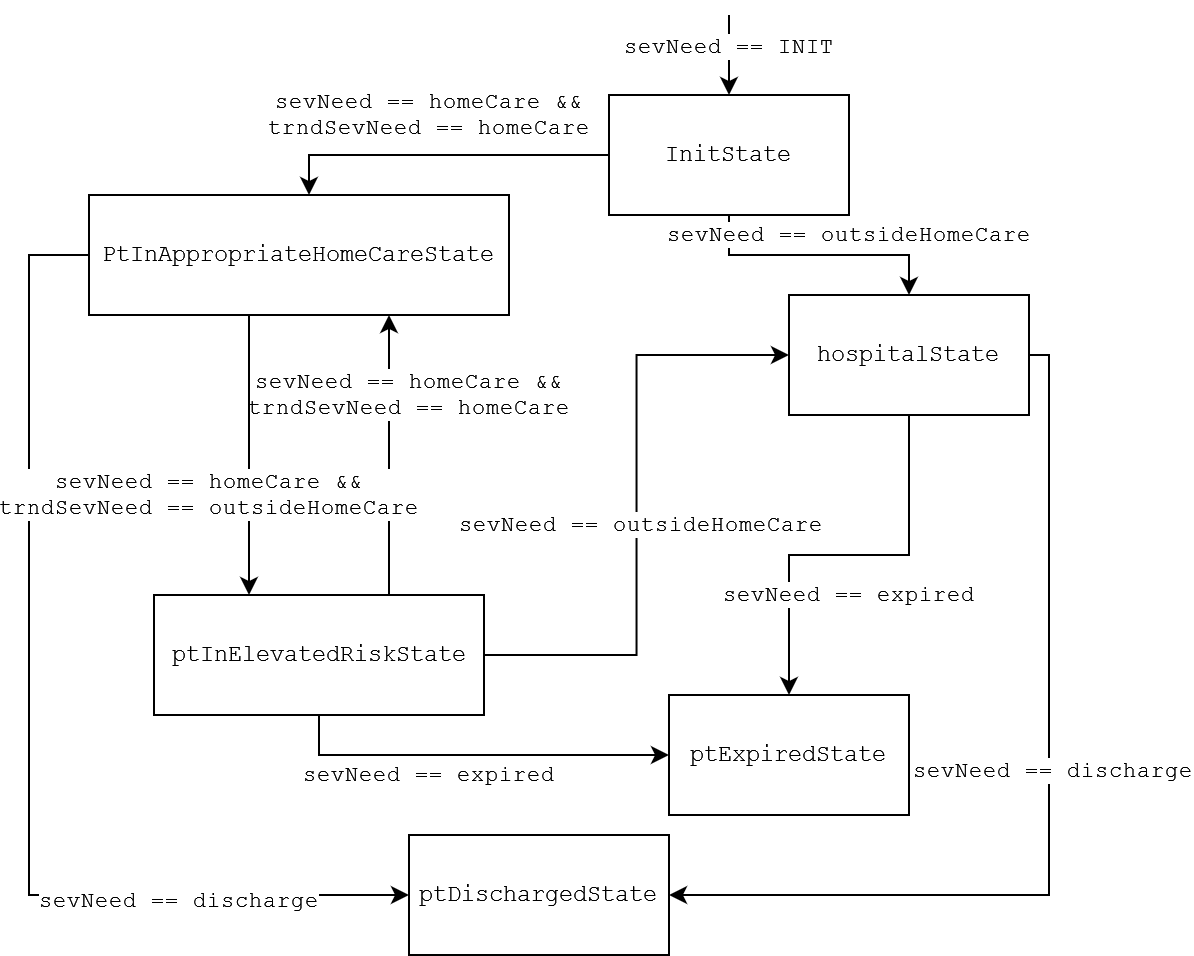
\includegraphics[width=\textwidth]{../figs/CWP/phware_CWP.png}
    \end{tabular}
  \end{center}
\caption{CWP state diagram for PHware example}
\label{fig:phware_cwp}
\end{figure*}

\figref{fig:longScaling2_bpmn} shows the BPMN of the fourth example. In this example, we show the scalability of the automation and verification process. This example contains a single actor with multiple decisions to make sequentially. We call this horizontal scaling. In this example, there are two sequential decisions. This number can be increased to push the limits of model checking in this context. \figref{fig:longScaling2_cwp} shows the corresponding CWP. The CWP here has just two states, only requiring that the BPMN execute to completion.

\begin{figure*}[t]
  \begin{center}
    \begin{tabular}{c}
        \includesvg[inkscapeformat=png, width=\textwidth]{../figs/BPMN/longScaling2_workflow.svg}
    \end{tabular}
  \end{center}
\caption{BPMN workflow for sequential scaling with two loops}
\label{fig:longScaling2_bpmn}
\end{figure*}

\begin{figure*}[t]
  \begin{center}
    \begin{tabular}{c}
        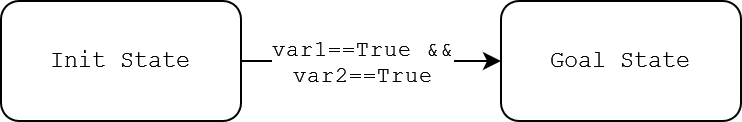
\includegraphics[width=\textwidth]{../figs/CWP/longScaling2_CWP.png}
    \end{tabular}
  \end{center}
\caption{CWP state diagram for sequential scaling with two loops}
\label{fig:longScaling2_cwp}
\end{figure*}

\figref{fig:wideScaling3_bpmn} shows the BPMN of the fifth example. This is also an example to show scalability. In this example, there are multiple actors, all with a single decision to make. In order to move throughIt is important to note that all of the actors interact with a single global state variable here. This type of scaling we will call vertical scaling. In this example, there are three actors \figref{fig:wideScaling3_cwp} shows the CWP for this example. Similar to the previous example, the CWP here only has two states. This ensures that each actor executes to completion.

\begin{figure*}[t]
  \begin{center}
    \begin{tabular}{c}
        \includesvg[inkscapeformat=png, width=\textwidth]{../figs/BPMN/wideScaling3_workflow.svg}
    \end{tabular}
  \end{center}
\caption{BPMN workflow for parallel scaling with three actors}
\label{fig:wideScaling3_bpmn}
\end{figure*}

\begin{figure*}[t]
  \begin{center}
    \begin{tabular}{c}
        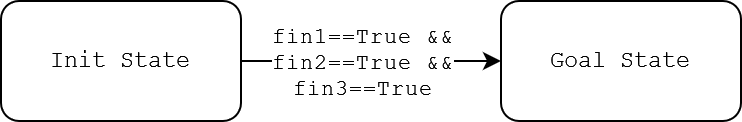
\includegraphics[width=\textwidth]{../figs/CWP/wideScaling3_CWP.png}
    \end{tabular}
  \end{center}
\caption{CWP state diagram for parallel scaling with three actors}
\label{fig:wideScaling3_cwp}
\end{figure*}

\figref{fig:verificationTimes} shows how long each model took to complete verification. Being the most simple example with no parallelism, the Face2Face verified the quickest, finishing in about two and a half minutes. The original Face2Face, with an error present, took slighly less time to verify. This is because, when the model checker detects an error, verification for a property can end sooner. If no errors are present, the entire state space must be searched. Next, BuyN'Sell, which introduces parallel execution, verified in four minutes and forty-one seconds. Finally, Phware, being the largest and most complex model, took eight minutes and forty-five seconds to verify.

\begin{figure*}[t]
  \begin{center}
    \begin{tabular}{c}
        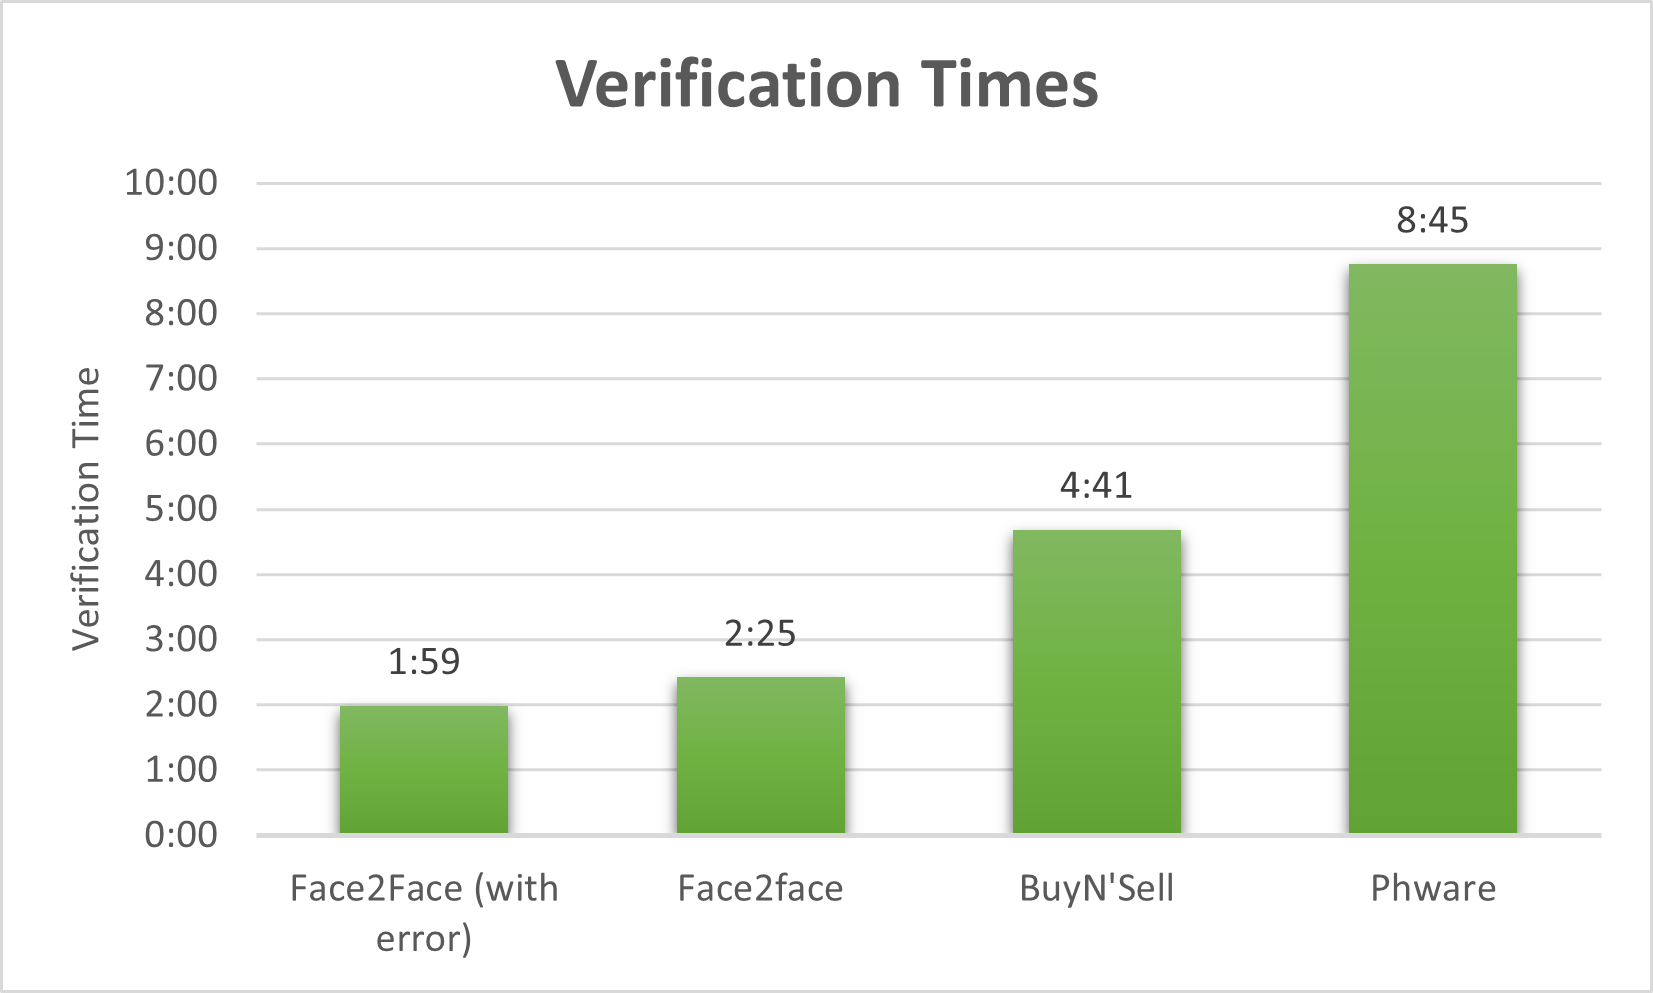
\includegraphics[width=\textwidth]{../figs/Data/Verification_Times.png}
    \end{tabular}
  \end{center}
\caption{Verification times for the four practical examples}
\label{fig:verificationTimes}
\end{figure*}

\figref{fig:longScalingVerificationTimes} shows the increase in verification time as the number of linear decisions increases in the sequential scaling BPMN example. The time requirement increases quadratically as the number of decisions increases. The largest example we tested had twenty sequential steps and took just over seven minutes to complete verification.

Several official BPMN best practice recommendations from BPM companies such as Camunda and Bizagi encourage BPMN modellers to keep diagrams as compact and simple as possible. If a model gets too large, it becomes difficult to read and understand. In those situations, it is best to identify parts of the model that can be separated into separate processes. Because of these recommendations, we believe that this model checking method scales sufficiently in sequential decisions.

\begin{figure*}[t]
  \begin{center}
    \begin{tabular}{c}
        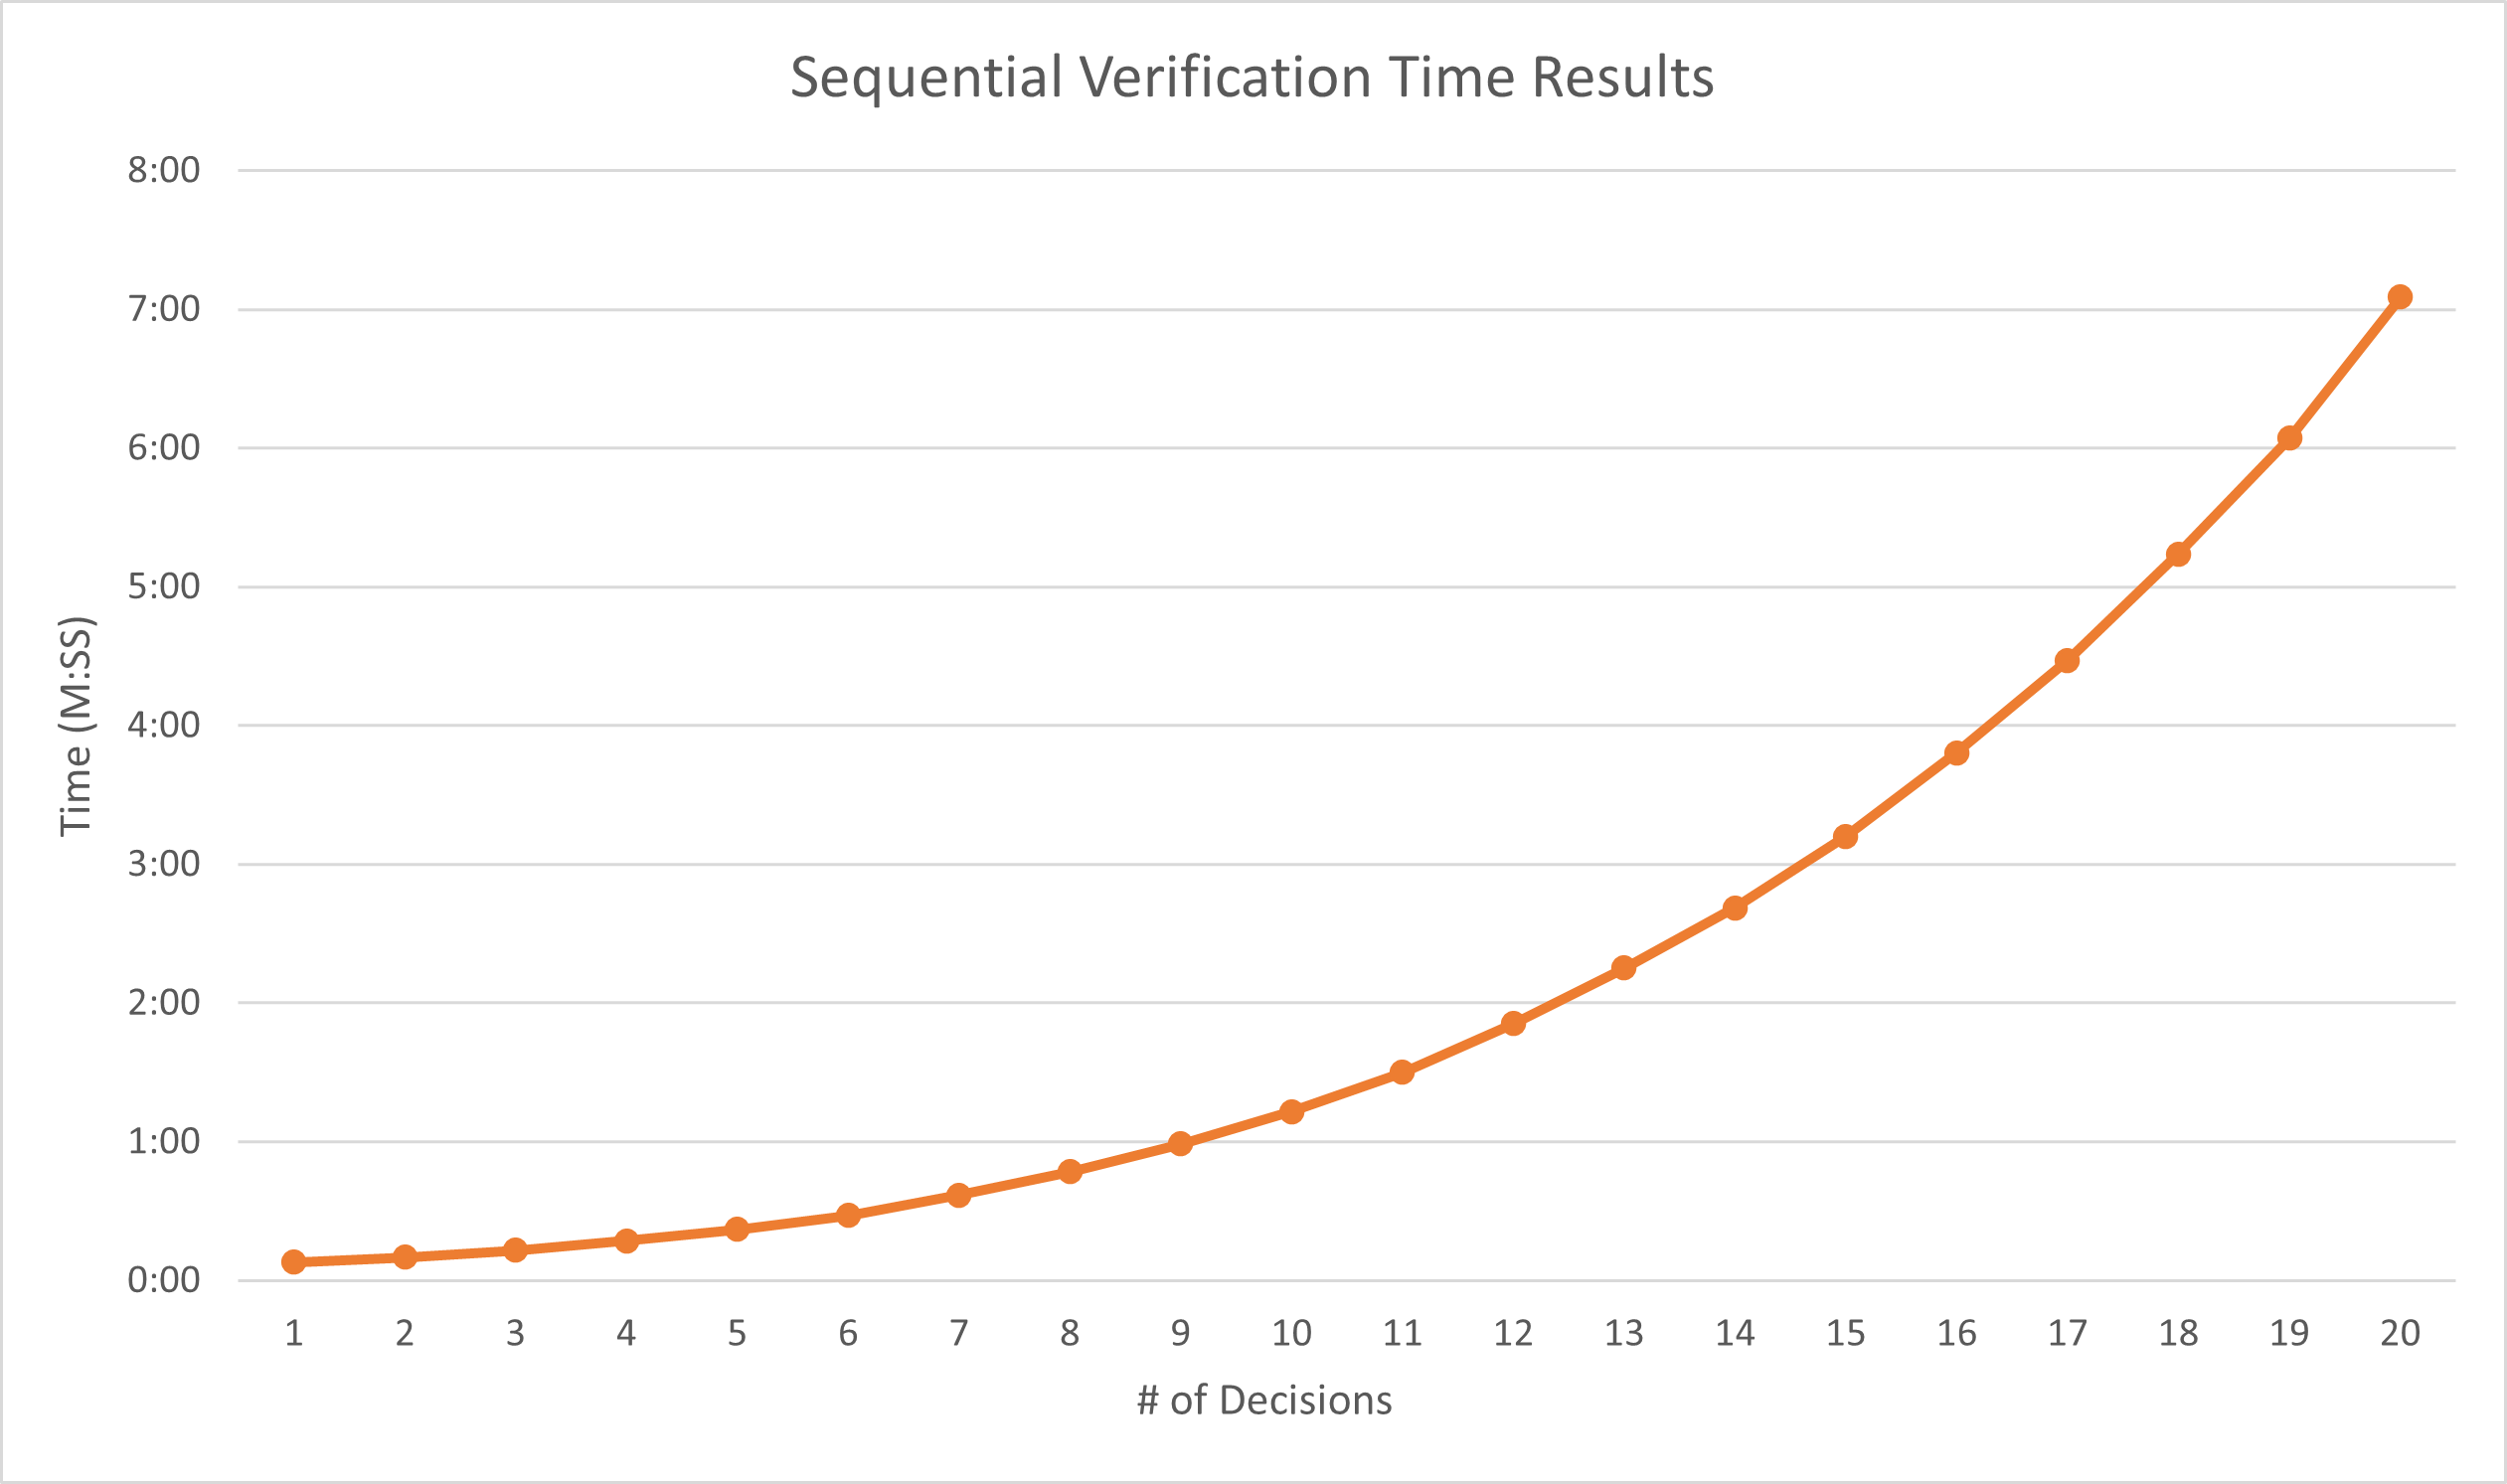
\includegraphics[width=\textwidth]{../figs/Data/Long_scaling_verification_times.png}
    \end{tabular}
  \end{center}
\caption{Verification times for the sequential scaling example by number of linear decisions}
\label{fig:longScalingVerificationTimes}
\end{figure*}

\figref{fig:wideScalingVerificationTimes} shows the increase in verification time as the number of synchronous actors increases in the parallel scaling BPMN example. Although the increase in verification time increases exponentially with the number of actors, it is important to note that this parallel example is the absolute worst case scenario in terms of parallelization. The structure of the parallel scaling example was created to introduce the maximum possible number of race conditions. This results in an incredibly fast increase in the number of states the model checker must search through.

In BPMN best practice, it is recommended to keep the number of parallel actors small in order to increase readability. Best practice often recommends subroutines and call activities in situations where a separate party is responsible for a large task. Short parallel tasks are not as significant because they result in considerably fewer race conditions as large tasks.

\begin{figure*}[t]
  \begin{center}
    \begin{tabular}{c}
        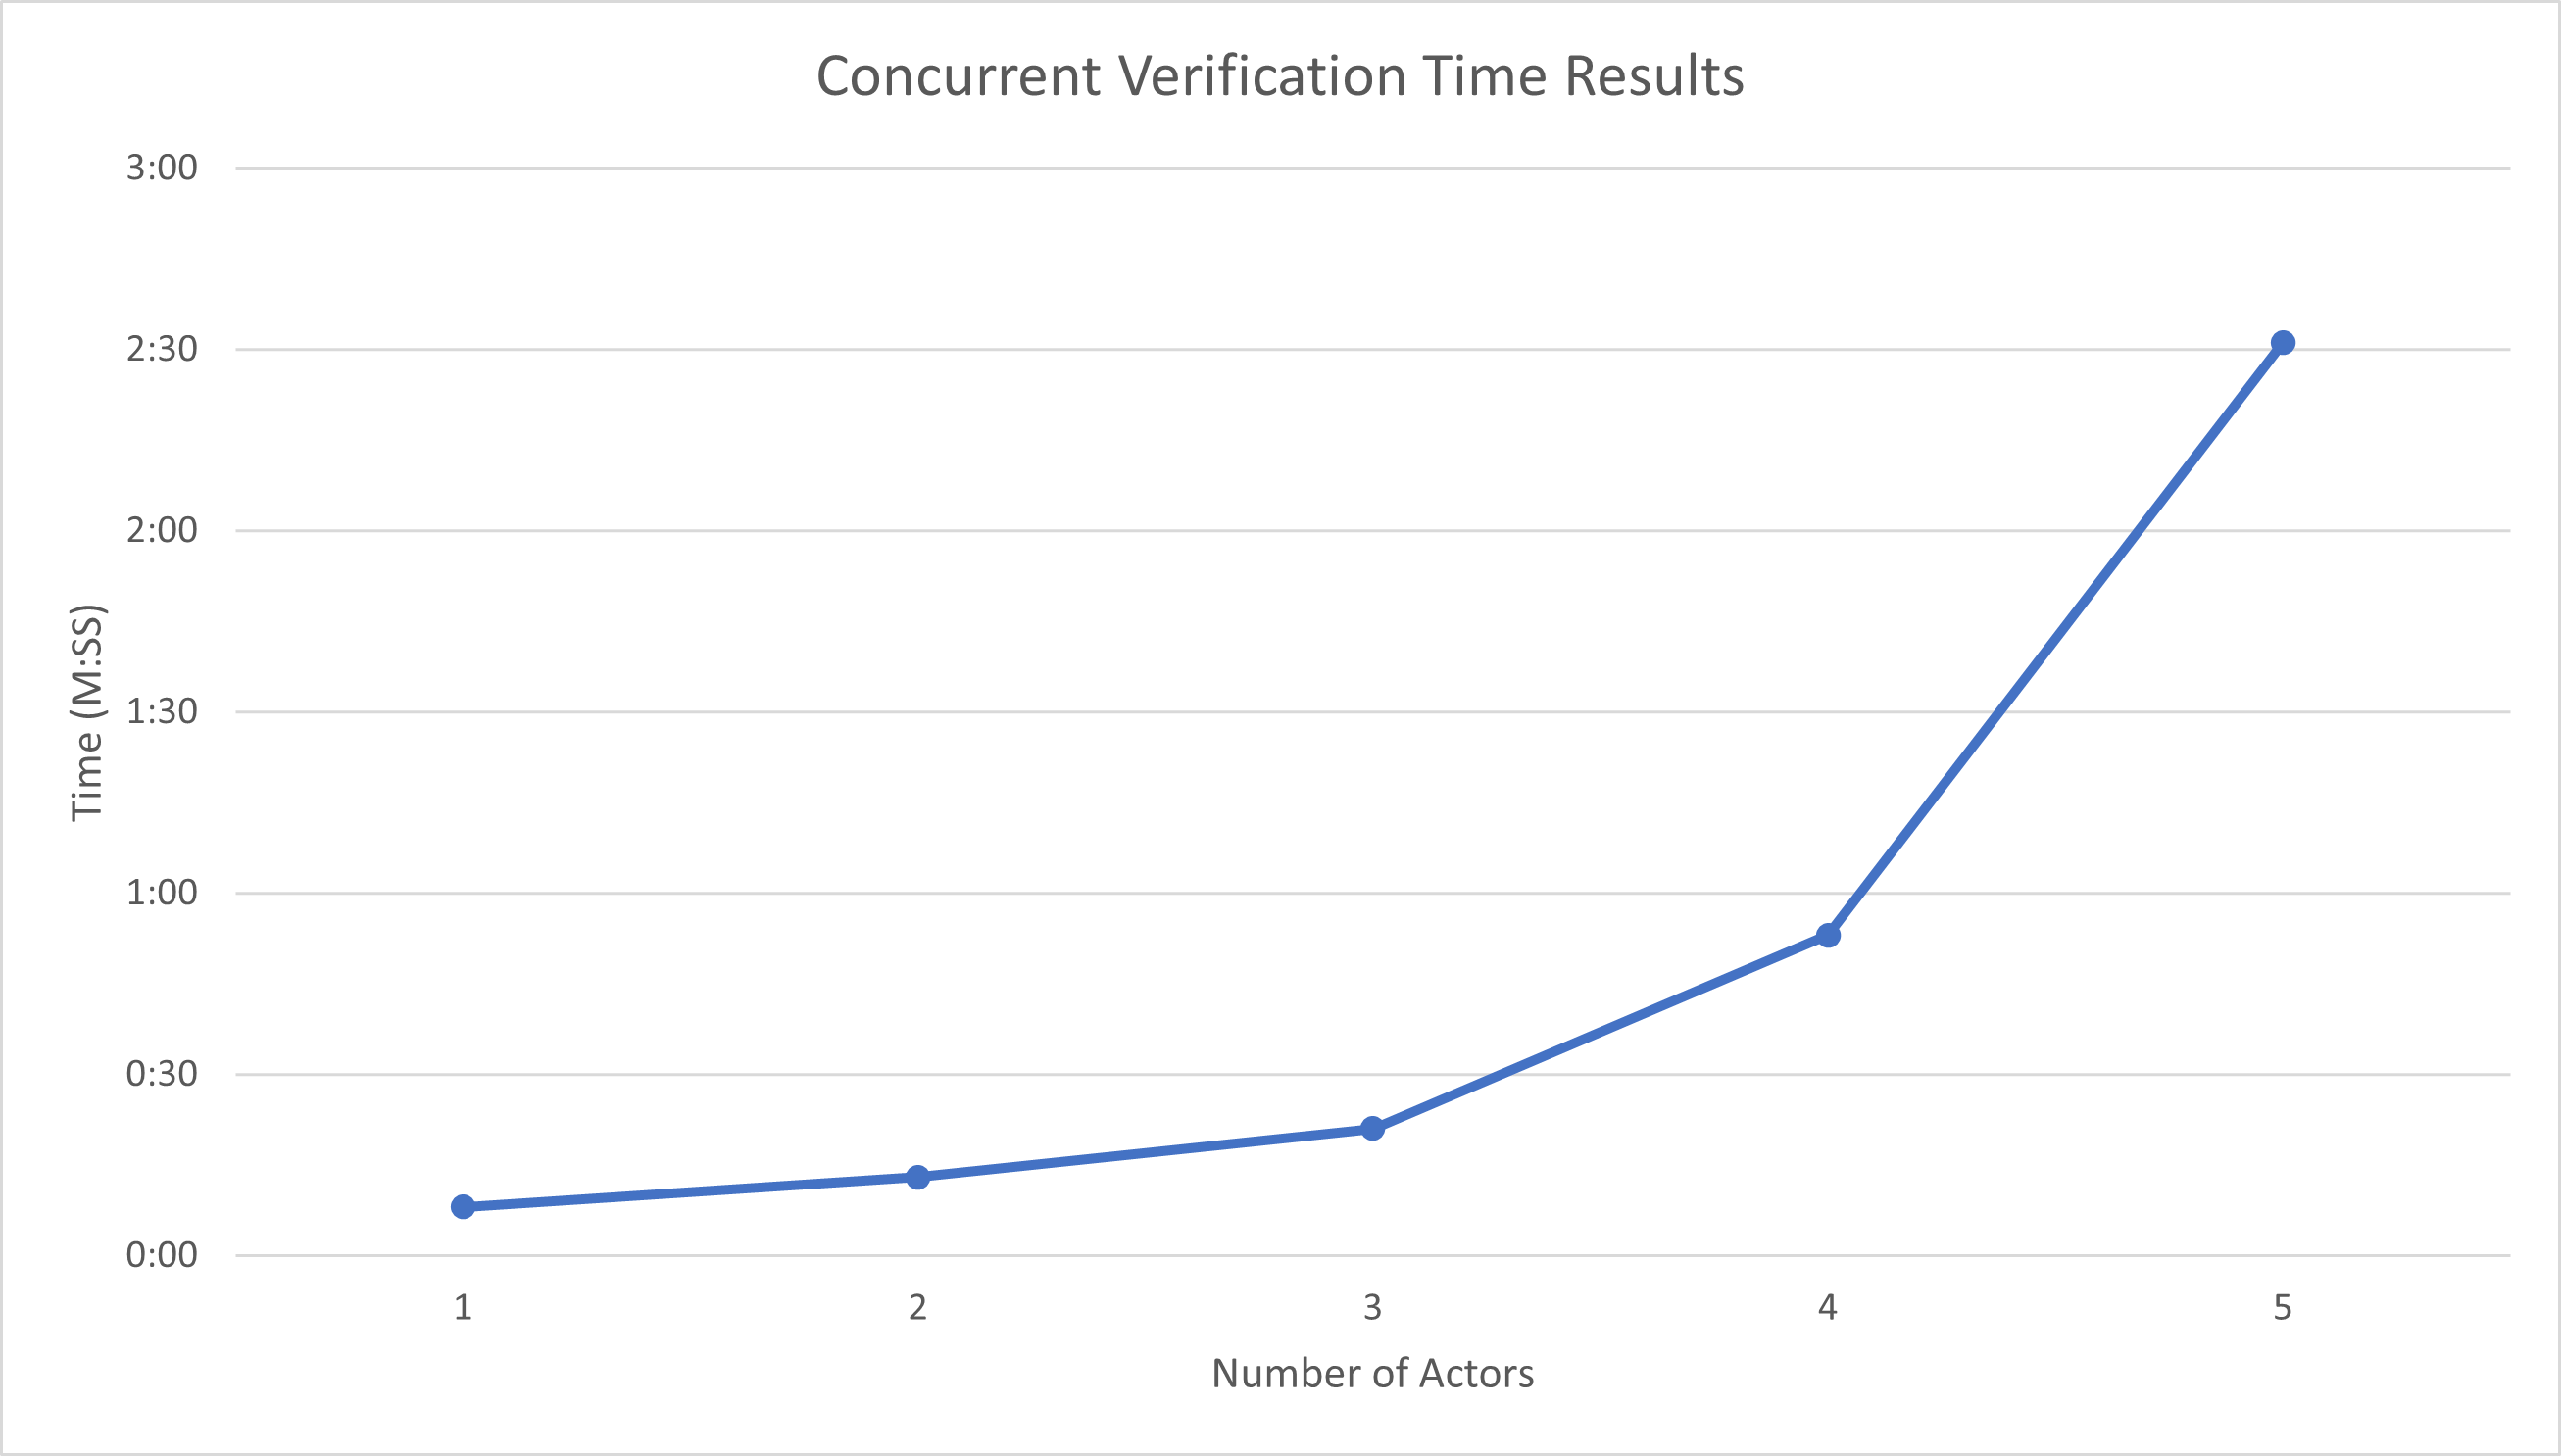
\includegraphics[width=\textwidth]{../figs/Data/Wide_scaling_verification_times.png}
    \end{tabular}
  \end{center}
\caption{Verification times for the parallel scaling example by number of concurrent actors}
\label{fig:wideScalingVerificationTimes}
\end{figure*}

.
.
.
.
.
.
.
.
.
.
